\chapter{Introduction}
\begin{quote}
\textit{The shape of the sea is always the same. Or rather it's always different, but in the same way.} --- Philip Marsden
\end{quote}

\section{The Atlantic Meridional Overturning Circulation}
\begin{itemize}
    \item Introduce the AMOC
    \item Explain how and why it's important
    \item Talk about how our understanding has changed in recent times
    \item Not a conveyor but variability and mesoscale features
    \item Introduce the idea that sub-mesoscale instabilities may play a role
    \item Talk about water mass formation, transformation, and diapycnal mixing
    \item Talk about the processes missing from the water mass budget.
\end{itemize}

\subsection{The Western Boundary Current Systems of  the Tropical Atlantic}

\subsection{The Irminger Current}

\section{Potential vorticity \& symmetric instability}
\begin{itemize}
    \item Describe the character of symmetric instability
    \item Introduce PV and the instability criteria
    \item Touch on links to inertial and gravitational instability but direct the reader to chapter 2 for more depth
    \item Lead into the subsections which describe ways of making potential vorticity negative.
\end{itemize}

Symmetric instability is a type of submesoscale instability that generates overturning cells in a plane perpendicular to a mean flow. The overturning cells tend to be oriented so that they are parallel to isopycnal surfaces, and so symmetric instability is often said to produce slantwise convection. Although the instability leads to mixing predominantly along isopycnals, it can also induce diapycnal mixing. Secondary shear instabilities further enhance this mixing.

Symmetric instability is intimately linked to the scaler quantity, Ertel potential vorticity. In the ocean this is defined as
\begin{equation}
    Q = (\mathbf{f} + \curl{\mathbf{u}})\cdot\grad b    
\end{equation}
where $\mathbf{f}$ is the planetary vorticity vector, $\mathbf{u}$ is the velocity field in the rotating frame of reference, and $b = -  g \flatfrac{\rho}{\rho_0}$ is the buoyancy field. $g$ is gravitational acceleration and $\rho_0$ is a constant reference density. One can interpret the potential vorticity as either the component of absolute vorticity normal to isopycnal surfaces and scaled by the isopycnal thickness, or the stratification along a vortex tube and scaled by the absolute vorticity of the vortex, with the former being the most common way of understanding the quantity.

In a fluid subjected to no momentum or buoyancy forcing, potential vorticity is materially conserved, i.e.
\begin{equation}
    \frac{DQ}{Dt} = 0 \, .
\end{equation}
This means if we follow an individual fluid parcel around we expect its potential vorticity to remain constant. This is a fundamental material invariant which arises from particle relabelling symmetries in the Lagrangian formulation of the equations of an IDEAL fluid.

If a fluid is subject to external or dissipative momentum and buoyancy forcings the conservation of potential vorticity  becomes
\begin{equation}
    \frac{DQ}{Dt} = \dot{\mathbf{\zeta}} \cdot  \grad{b} + \mathbf{\zeta} \cdot \grad{\dot{b}}
\end{equation}
where $\mathbf{\zeta}$ is the absolute vorticity of the field and a $\,\cdot{}\,$ above a quantity represents its material derivative.

A necessary but not sufficient condition for the excitement of symmetric instability is that the vertical component of planetary vorticity and the potential vorticity of a fluid have opposite signs. Mathematically we require that
\begin{equation}
    \label{eq:PVConservation}
    f Q < 0 \, ,
\end{equation}
where $f$ is the vertical component of the planetary vorticity vector, also known as the Coriolis parameter. Waters which satisfy this instability criterion are often described as having anomalous potential vorticity.

The overturning cells generated during the excitement of symmetric instability causes the mixing of waters with anomalous potential vorticity. The momentum and stratification of the fluid are reconfigured by this mixing, producing waters with potential  vorticity of approximately zero. This corresponds to the absolute vorticity vector being parallel to isopycnal surfaces.

Consider now a fluid initially stable to symmetric instability. For it to become symmetrically unstable we must make the quantity $fQ$ negative. There are then two distinct ways to generate symmetric instability in such a fluid: the first is to change the sign of the planetary vorticity, and the second is to change the sign of the potential vorticity.

\subsection{Ekman driven symmetric instability}
\begin{itemize}
    \item can diffusion generate symmetric instability?
\end{itemize}

\subsection{Cross equatorial symmetric instability}
At the equator planetary vorticity changes from being positive in the northern hemisphere to negative in the southern hemisphere. If we consider a fluid parcel originating in one hemisphere, its potential vorticity will typically match the planetary vorticity so as to ensure symmetric stability. We can than imagine advecting this fluid parcel across the equator. As potential vorticity is materially conserved and planetary vorticity changes sign at the equator, we would expect the symmetric instability criterion to be satisfied in the new hemisphere.

This mechanism does not involve buoyancy or momentum forcing, processes which typically must occur in either a surface or bottom boundary layer. This means symmetric instability resulting from a change in sign of planetary vorticity may occur in the ocean interior and has a distinct character when compared to boundary layer instability. A number of recent observational and theoretical studies have investigated the excitement of symmetric instability resulting from the cross-equatorial change in sign of planetary vorticity, notably CITATIONS. These studies have, however, focused on weak circulations in the ocean interior as opposed to vigorous western boundary currents. In these western boundary currents there is a constant supply of waters with large magnitude, anomalous potential vorticity. These equatorial western boundary currents are rich with temporally varying features, such as mesoscale eddies which interact differently with symmetric instabilities depending on the flow regime.

\begin{figure}
    \centering
    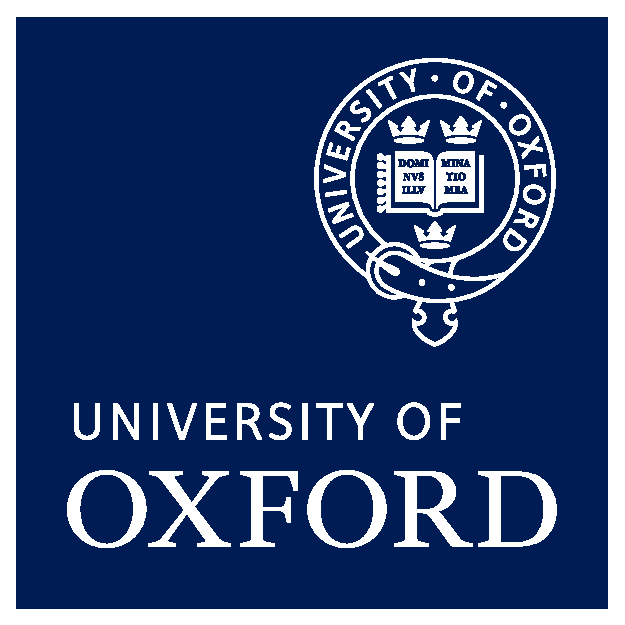
\includegraphics[width=0.5\textwidth]{oxlogo.eps}
    \caption{Caption}
    \label{fig:my_label}
\end{figure}